\documentclass[conference]{IEEEtran}
\IEEEoverridecommandlockouts
% The preceding line is only needed to identify funding in the first footnote. If that is unneeded, please comment it out.
\usepackage{cite}
\usepackage{amsmath,amssymb,amsfonts}
\usepackage{algorithmic}
\usepackage{graphicx}
\usepackage{textcomp}
\usepackage{xcolor}
\usepackage{subfigure}
\usepackage{url}
\usepackage{xurl}% Required for \url command
\def\BibTeX{{\rm B\kern-.05em{\sc i\kern-.025em b}\kern-.08em
    T\kern-.1667em\lower.7ex\hbox{E}\kern-.125emX}}

\begin{document}

\title{A Sweat-Based Wearable Sensor for Real-Time Lactate and Glucose Monitoring in Endurance Athletes}

\medskip

\author{\IEEEauthorblockN{Elliot Metcalf}
\IEEEauthorblockA{\textit{Department of Electrical and Computer Engineering} \\
\textit{Rice University}\\
Houston, USA \\
etm2@rice.edu}
\and
\IEEEauthorblockN{Priyanka Amalkar}
\IEEEauthorblockA{\textit{Department of Electrical and Computer Engineering} \\
\textit{Rice University}\\
Houston, USA \\
pa52@rice.edu}
\and
\IEEEauthorblockN{Zhenya Liu}
\IEEEauthorblockA{\textit{Department of Electrical and Computer Engineering} \\
\textit{Rice University}\\
Houston, USA \\
zl181@rice.edu}
}

\maketitle

\begin{abstract}
This project explores a sweat-based wearable sensor for real-time monitoring of lactate and glucose in endurance athletes during training. Monitoring these analytes can help endurance athletes optimize their workouts and ultimately enhance their athletic performance. However, existing commercial solutions are invasive (blood-based), expensive, and the slow nature of the testing process causes undesired disruption during an activity. To address these limitations, the design team conducted extensive research on existing sweat-based sensing devices and developed an outline of a wearable system that integrates a custom sensor, a flexible circuit board, and microfluidic channels. The system can interact with a smart watch or smartphone via Bluetooth, providing athletes with near-real-time biochemical feedback.
\end{abstract}

\smallskip

\section{Introduction}
During endurance and sports training, it is important to track different analytes to determine physiological changes. Knowing the impact of these fluctuating biomarkers can reveal ways to enhance athlete performance. Lactate levels are key for athletes to track since increasing levels are indicative of anaerobic metabolism, which causes muscle fatigue and cramping. Determining their lactate threshold allows the athlete to understand their optimum training and monitor fatigue to improve performance. Glucose is another important analyte to track since decreasing glucose levels directly correspond to decreasing energy levels. Alerting the athlete when their blood sugar decreases will allow them to time their food intake to maintain stable energy levels throughout the training session. Due to differences in types of sweat composition, we will be focusing on sweat collected during exercise.
\bigskip

\section{Method}

\smallskip

\subsection{Device}
The methodology for developing our wearable biosensor device involved a multidisciplinary, iterative design process including sensor fabrication and the integration of a flexible PCB with a microfluidic patch for real-time analyte monitoring. At our current stage, we first prototyped the electronic circuitry using an Arduino-based system, where an 8-bit PWM signal was generated to produce a linear-like analog voltage after being smoothed by an RC filter. The setup served as the digital-to-analog converter due to Arduino R3 lacking true DAC. The PWM frequency was modified to approximately 31.4 kHz by changing the divider factor to 1 in Equation (1), where the clock frequency for Arduino R3 UNO board and is 16 MHz in this case. It ensures smooth voltage transitions and avoids disrupted DC sweep.

\begin{equation} f_{PWM} = \frac{f_{clk}}{2 \times divider \times 255}\end{equation}

\begin{figure}[hptb]
    \centering
    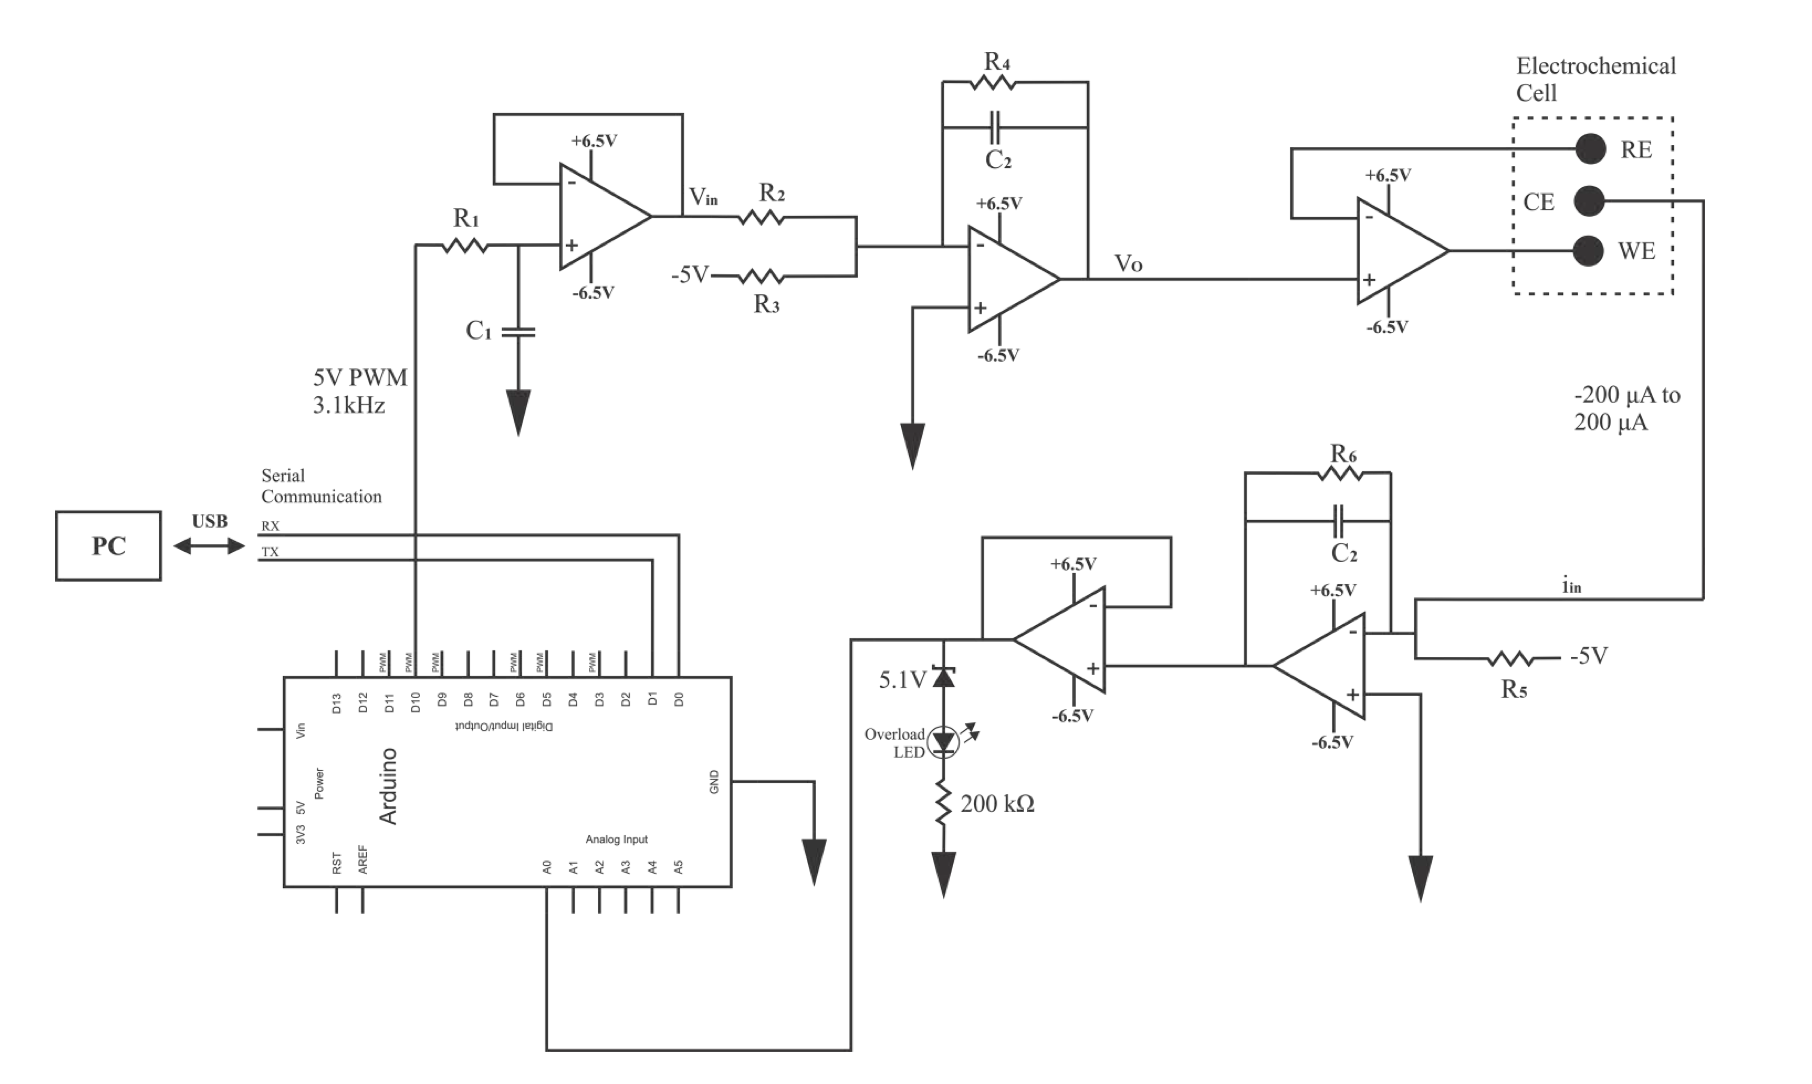
\includegraphics[width=0.45\linewidth]{fig1.png}
    \caption{Full schematic design of the potentiostat including the Arduino board}
    \label{fig}
\end{figure}
\smallskip

\smallskip
\begin{figure}[hptb]
    \centering
    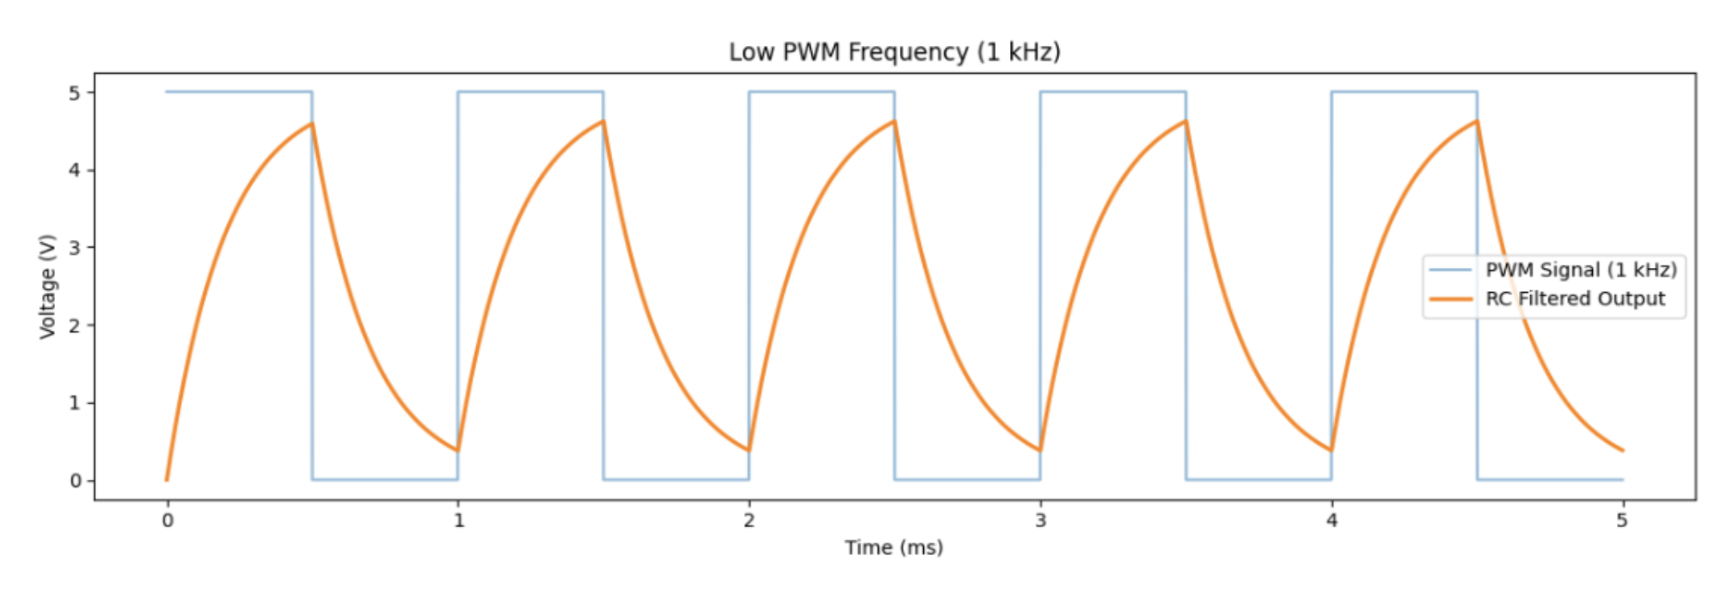
\includegraphics[width=0.45\linewidth]{fig2.png}
    \caption{RC filtered Output of PWM (31 kHz)}
    \label{fig}
\end{figure}
\smallskip

\begin{figure}[hptb]
    \centering
    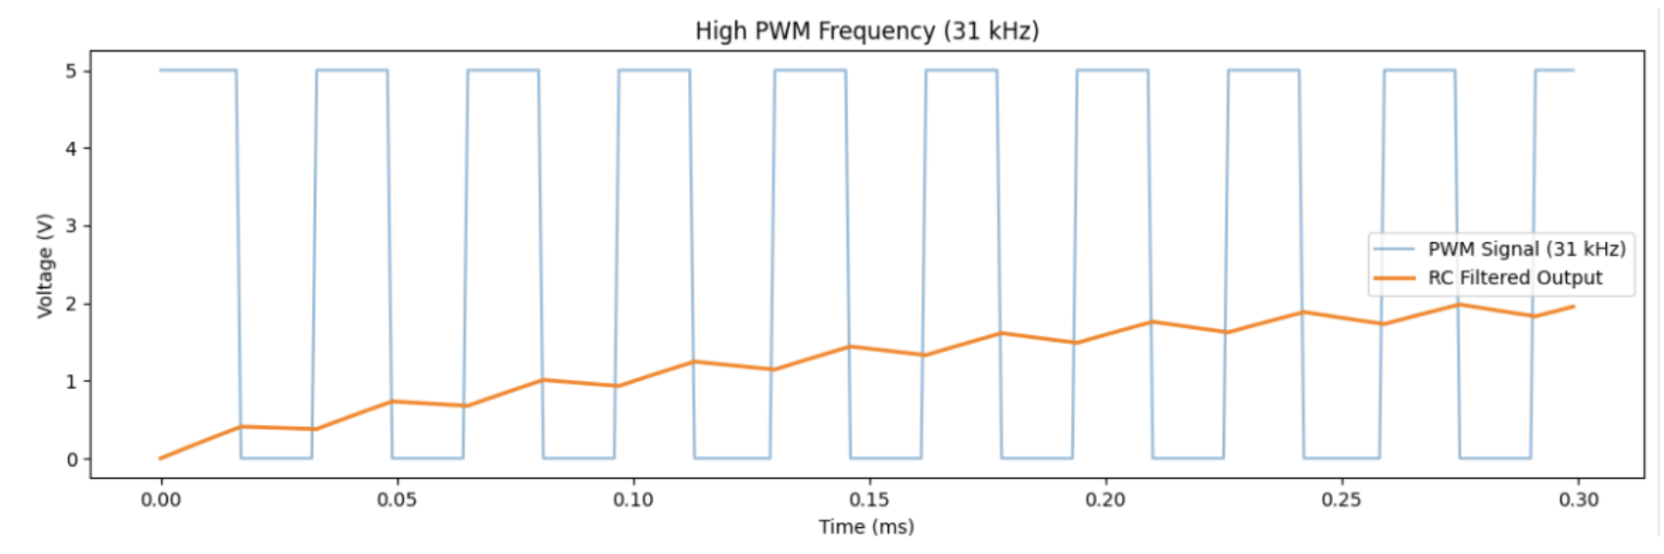
\includegraphics[width=0.45\linewidth]{fig3.png}
    \caption{RC filtered Output of PWM (1 kHz)}
    \label{fig}
\end{figure}
\smallskip

Then a transimpedance amplifier circuit was implemented to convert the current flow at the counter electrode into a voltage before being transmitted to a 10-bit ADC of the Arduino board. Lastly, The result will be printed out via Arduino port. The test through CV allowed us to validate sensor performance and fine-tune the electronic parameters. Once the electrical functionality of the prototype circuit was verified on a rigid PCB, the next stage includes transferring the design to a flexible PCB to ensure the adaptability and robustness of the system for wearable applications. 

\subsection{Sensor}
The sensor is made up of a reference electrode, two working (lactate and glucose) electrodes, and a counter electrode. The reference electrode provides a stable, known potential. The working electrode is where the reaction takes place and current is measured. The counter electrode completes the circuit and undergoes the opposite reaction from the working electrode.
The screen printing method was chosen because it is easy to develop the sensors and reprint if design changes are made. In the screen printing process, two inks are used. The first is silver (Ag) that makes up the majority of the counter and working electrodes, and the entire reference electrode. Silver is chosen because of its strong electrical conductivity. The main part of the counter electrode and working electrodes are printed in carbon that has been prepared with prussian blue.
This electrochemical sensor works by detecting changes in current that are proportional to analyte changes in the sweat. The lactate working electrode is modified using the lactate oxidase enzyme, immobilizing it onto the surface of the electrode through curing. Similarly, the glucose working electrode is modified using glucose oxidase. When the enzyme reacts with its respective analyte, it produces hydrogen peroxide (H2O2). The prussian blue in the carbon ink is highly selective towards hydrogen peroxide and undergoes reduction when reacted with H2O2. The current changes from this reaction are then picked up by the working electrode when voltage is applied to read the current measurements, which are proportional to the analyte concentration.

\begin{figure}[htbp]
    \centerline{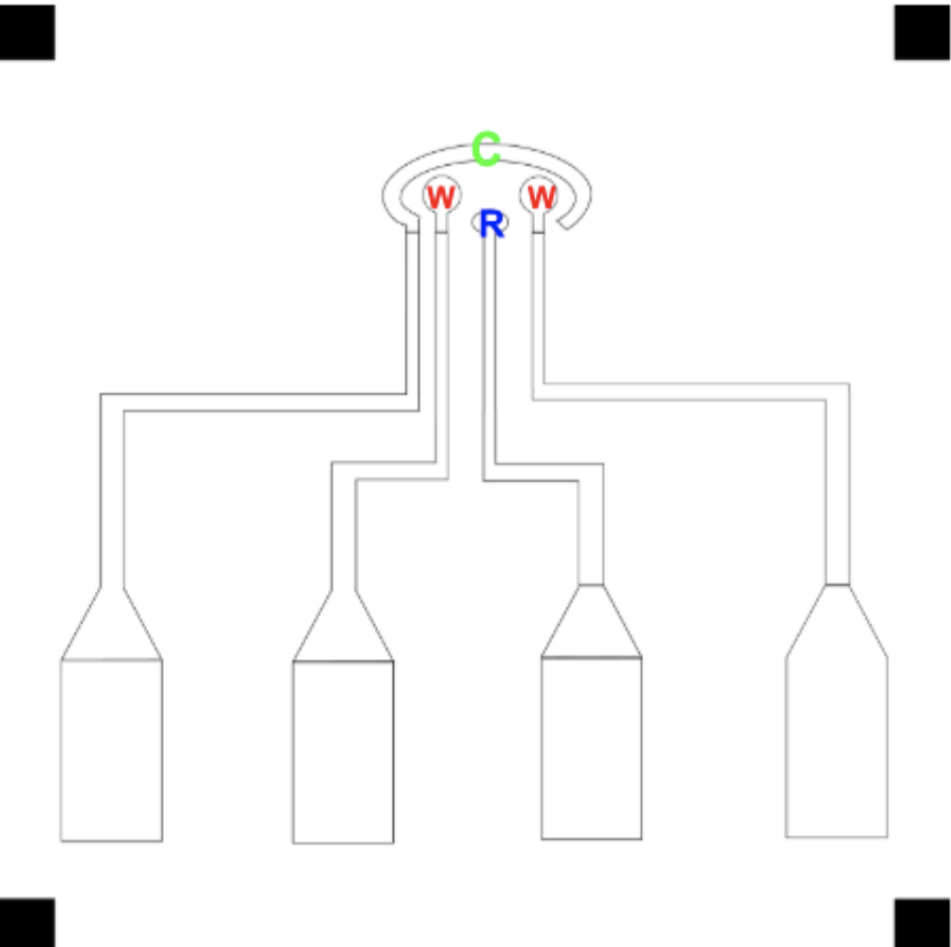
\includegraphics[width=0.45\linewidth]{fig4.png}}
    \caption{Final sensor design with labeled counter, reference, and working electrodes}
    \label{fig}
\end{figure}

\smallskip
The specifications used to design the above sensor are as follows. Both working electrodes share one counter and one reference electrode. Both working electrodes are equidistant from the counter electrode to ensure that there is an equal current distribution. The counter electrode and the area within it must be less than 11mm by 5mm to ensure that there is an optimum sweat flow in the microfluidics reservoir. The circular diameter of the working electrodes will later be optimized once the calibration curve test is conducted. 
The method for screen printing our sensor design is as follows. First, sheet of kapton is layered onto a clear base (acetate). Using the Cricut, the sensor design is printed onto the kapton. The kapton parts that must be silver (reference, and counter/working leads) are peeled off. A layer of silver ink is added by placing some ink at the top of the design and dragging it downwards with a squeegee. It is cured in the oven at 120 Celsius for 15-20 min. The kapton parts that must be carbon are peeled off. To protect the silver ink surfaces, a mask can be added on top before adding a layer of carbon ink. Make sure to have the carbon ink overlap slightly with the silver ink for the counter and working electrodes. It is cured again in the oven at 120 Celsius for 15-20 min. After removing the rest of the kapton from the design, the final screen printed sensor is left on the base. Using this design, two batches of 8 sensors each were screen printed.
A preliminary test to confirm if the sensor has good connectivity after printing is resistance measurement. For this test, the positive and negative leads of the ohmmeter touch the farthest carbon and silver points of the working electrode. If the electrode has good electrical conductivity, the resistance should be low, ideally less than 1k Ohm. This process is repeated for the other working and counter electrodes. The main reason why resistance could be high in this test is if there are gaps in the ink (could be caused by skipped ink during printing or ink lifting when removing the kapton), creating breaks in the electrode. The 16 sensors were resistance tested. Of the 8 in the first batch, 3 of them passed while 5 failed. In the second batch of 8, 5 passed while 3 failed.
During the cyclic voltammetry (CV) test, the solution may come in contact with the silver area,  causing an unwanted reaction and distorted CV results. An isolation solution can be created to limit the area of solution contact to the tips of the electrodes. Styrene Ethylene Butylene Styrene (SEBS) is a thermoplastic elastomer that is dissolved in tetrahydrofuran (THF) to create a viscous solution that can be pipetted onto the sensor. One part of SEBS to nine parts of TFH were used to create the solution. Once the solution has dried on the sensor, resistance testing must be done again to ensure that there was no disruption to the ink during pipetting the isolation solution. Of the 8 sensors that passed initial resistance testing, 3 passed resistance testing after the isolation solution was applied. 
\smallskip
\begin{figure}[hptb]
    \centering
    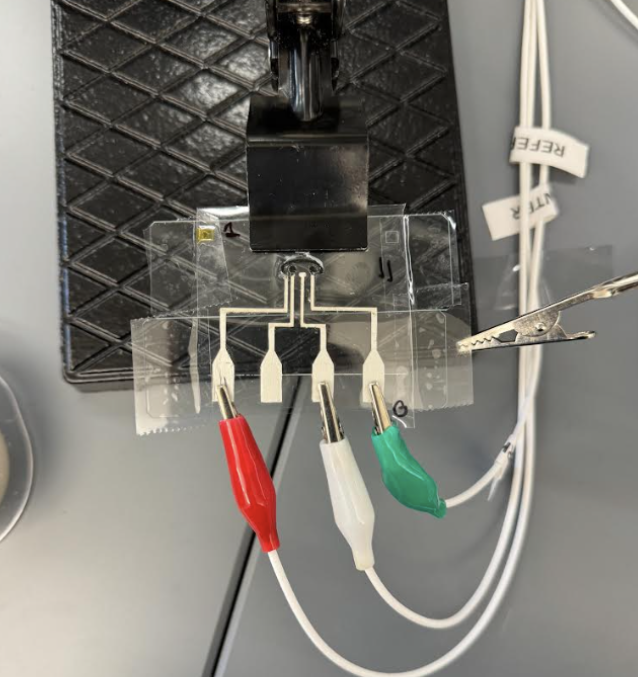
\includegraphics[width=0.45\linewidth]{fig5.png}
    \caption{CV test setup with sensor 1}
    \label{fig}
\end{figure}
\smallskip
Cyclic voltammetry is done to ensure that a good signal is being captured by the electrodes before moving onto electrode modification. A solution of phosphate buffered saline (PBS) is used due to its similarity of salt and pH to biofluid composition. Using a bench-top potentiostat, a graph is generated that quantifies current change as the prussian blue undergoes a redox reaction with H2O2 in the solution. An ideal graph has two peaks, one positive peak for oxidation, and one negative peak for reduction. If there is more than one peak, in the positive and/or negative peaks, the CV results have been distorted, likely due to other unwanted reactions taking place.
\smallskip
\begin{figure}[hptb]
    \centering
    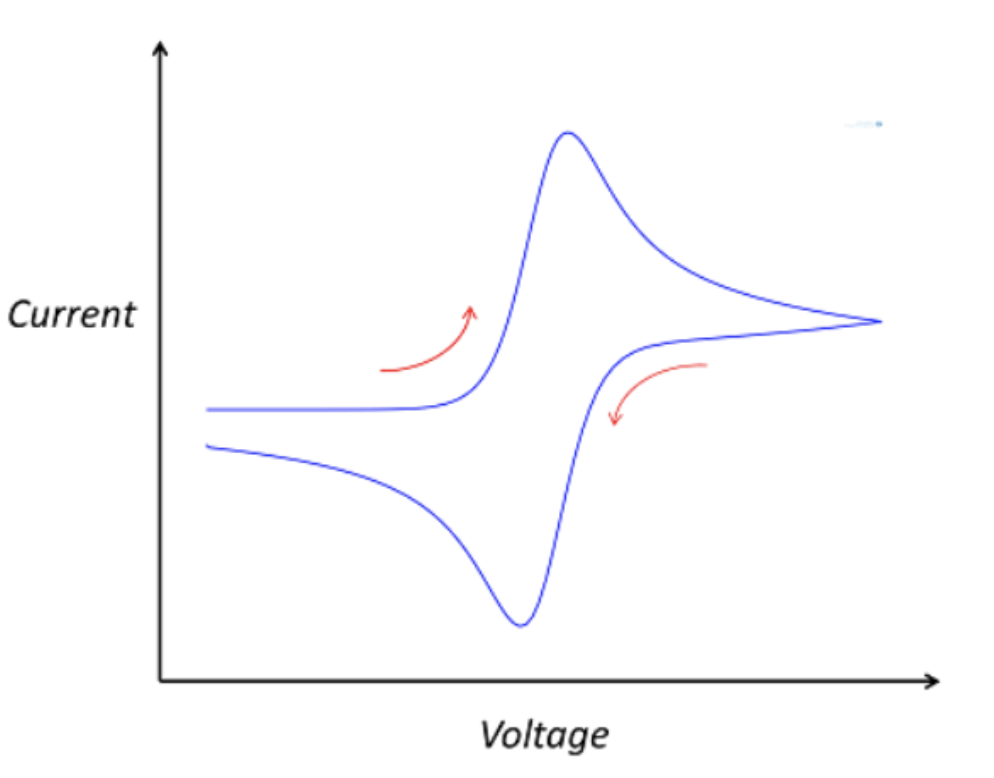
\includegraphics[width=0.45\linewidth]{fig6.png}
    \caption{Ideal CV graph shape}
    \label{fig}
\end{figure}

\smallskip

\subsection{Microfluidics}
The microfluidic system was designed to transport sweat from the skin to the custom glucose and lactate sensor for measurement. The initial microfluidic layout was created using AutoCad and the layout was based on our research of microfluidic systems in similar devices. To assess whether the layout was suitable for our project, SimScale was used for computational fluid dynamics (CFD) simulations. These simulations modeled expected sweat flow behavior through the channels and the reservoir and highlighted areas where adjustments were needed.
Following sensor modifications and feedback from advisors, the layout was refined to improve the rate of fluid delivery and accommodate sensor integration. After each design modification, further simulations were conducted to validate the changes and ensure consistent flow across the sensing reservoir.
Two different designs were chosen for testing. Microfluidic molds were fabricated for each using a resin-based 3D printer. Polydimethylsiloxane (PDMS) was prepared by mixing the polymer base and the curing agent in a 20: 1 ratio, then poured over the 3D printed mold and cured at 70 ° C for three hours to form the microfluidic chip. Two approaches were used to obtain the PDMS chips from the molds, as we anticipated difficulties working with an extremely thin layer of PDMS. The first mold was made with excess height, and the amount of PDMS required to fill it to a height of 300 microns was calculated and poured in. The second mold had no excess height. PDMS was applied over the mold, and a scraper was used to distribute it evenly over the entire surface.
\bigskip

\section{Results}

\smallskip

\subsection{Device}
The complete integration of the prototype and CV testing has not yet been completed, so real results are not available at this stage. However, preliminary work on individual modules has shown that our code implementations are working as intended. We have successfully validated the PWM generation, ADC conversion, and voltage sweep in code implementation shown in the Fig 7. and Fig 8. Once all the remaining parts arrive, we will proceed with connecting the full schematic of potentiostat prototype. 

\smallskip
\begin{figure}[hptb]
    \centering
    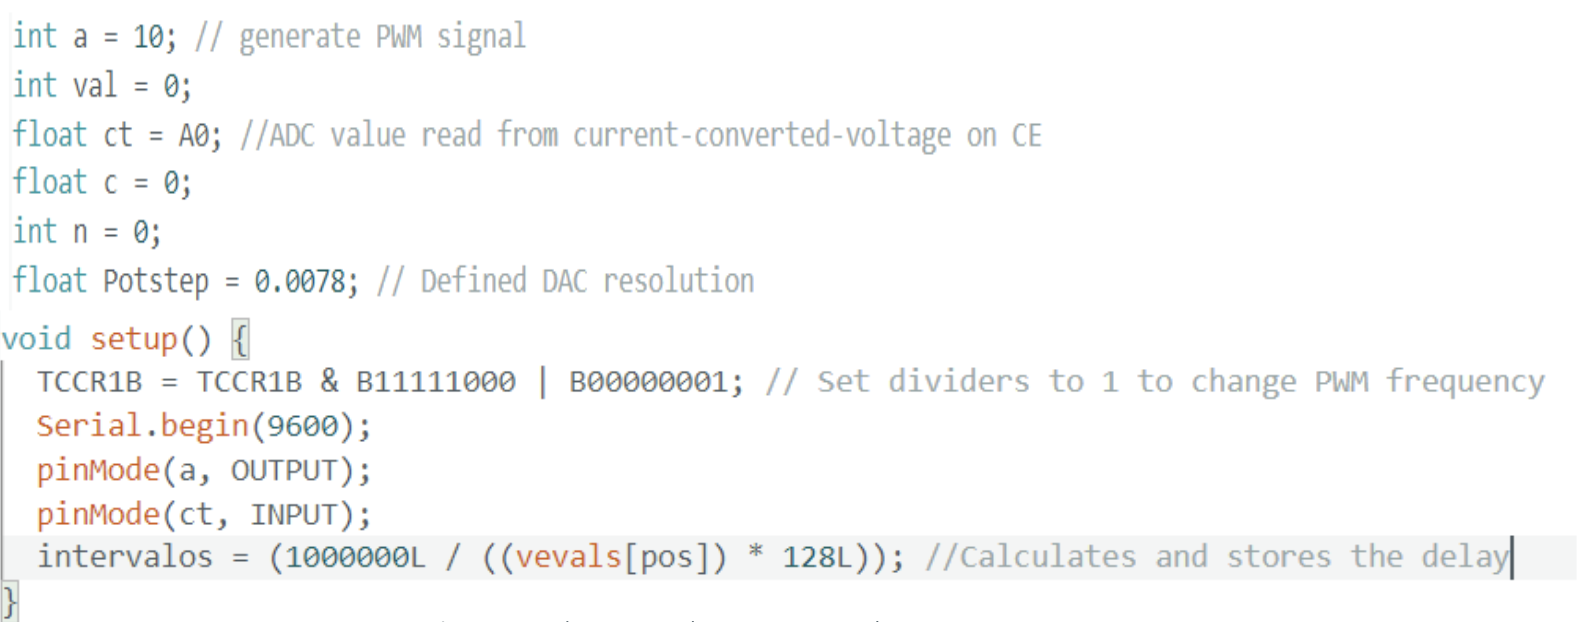
\includegraphics[width=0.45\linewidth]{fig11.png}
    \caption{Arduino IDE code parameter initialization}
    \label{fig}
\end{figure}
\smallskip

\smallskip
\begin{figure}[hptb]
    \centering
    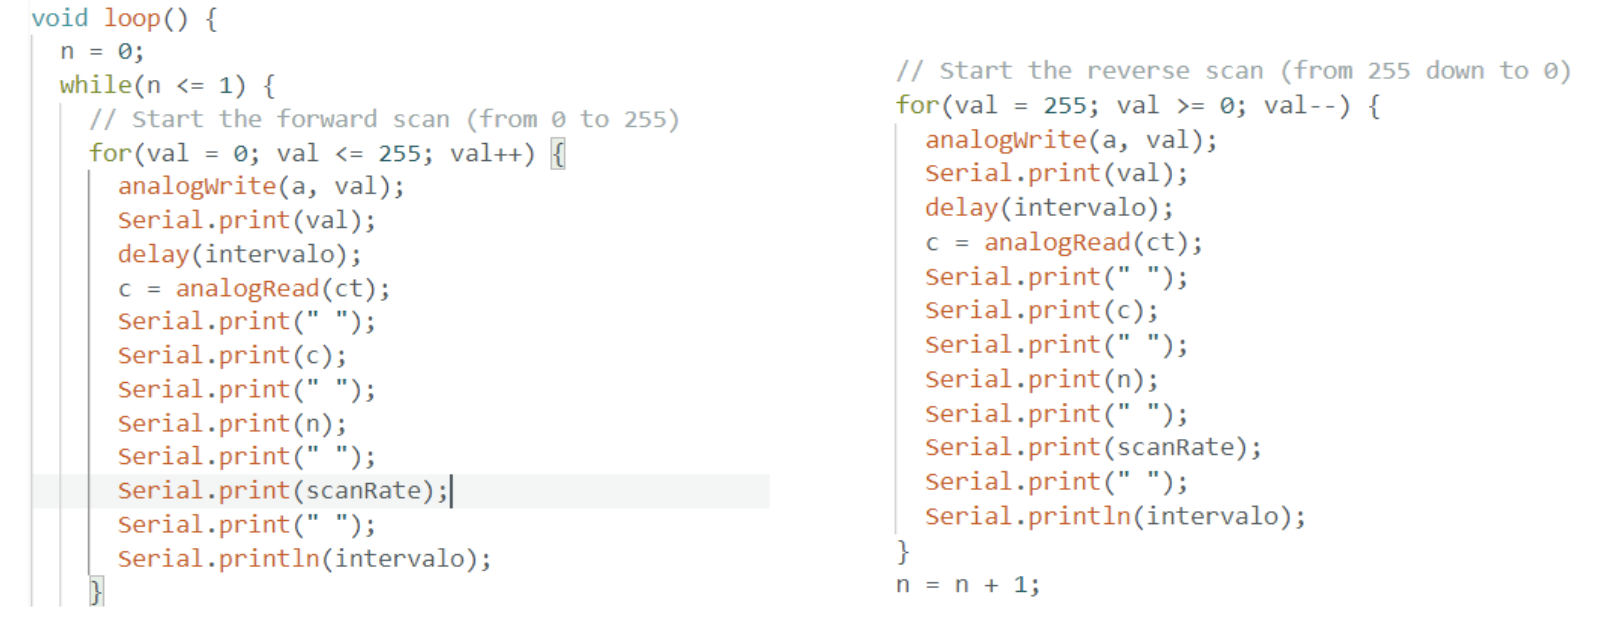
\includegraphics[width=0.45\linewidth]{fig12.png}
    \caption{Main loops containing forward and reverse scan}
    \label{fig}
\end{figure}
\smallskip

\subsection{Sensor}
% \begin{figure}[hptb]
%     \centering
%     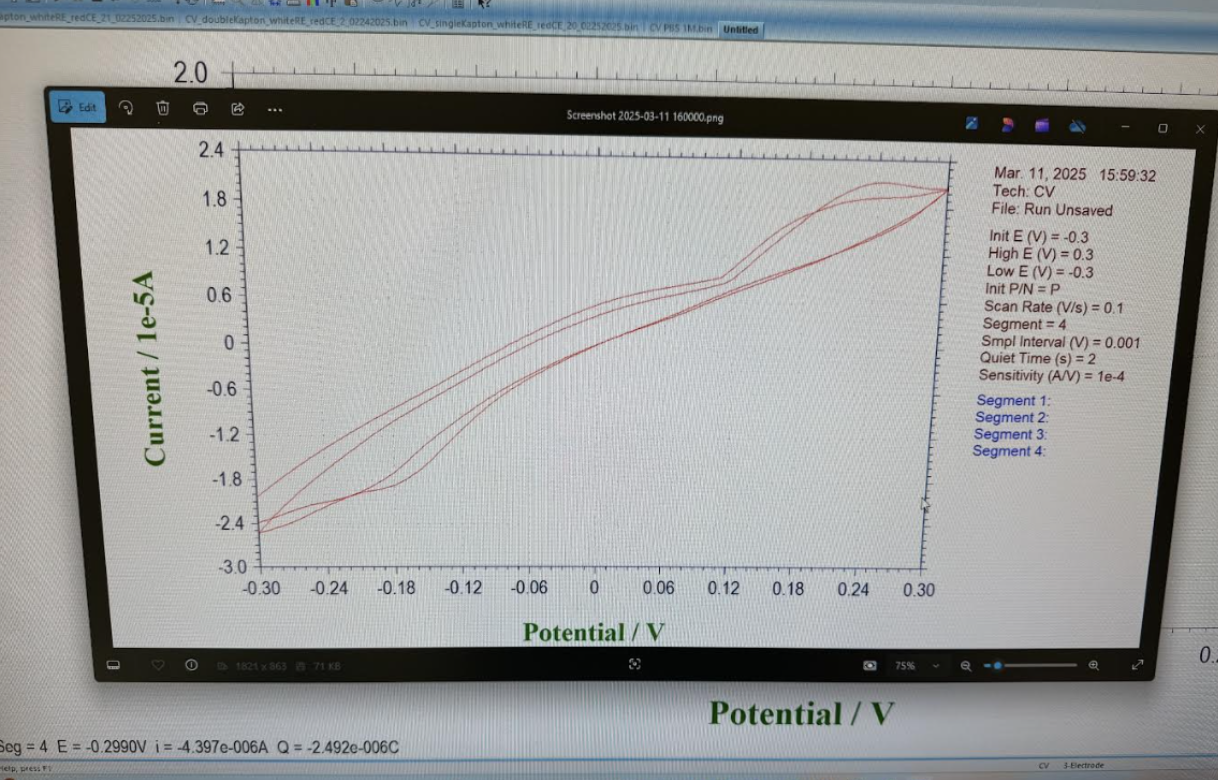
\includegraphics[width=0.45\linewidth]{fig7.png}
%     \caption{Sensor 1 CV results}
%     \label{fig}
% \end{figure}


\begin{figure}[hptb]
    \centering
    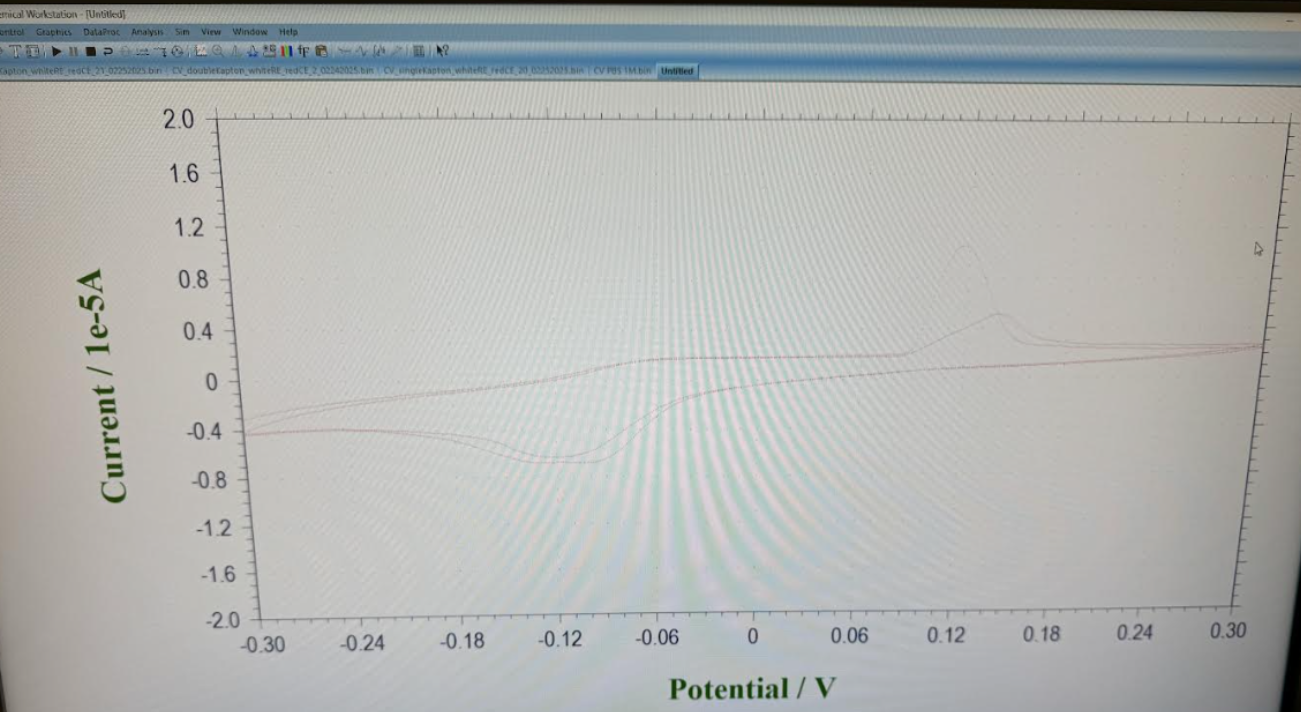
\includegraphics[width=0.45\linewidth]{fig8.png}
    \caption{Sensor 2 CV results}
    \label{fig}
\end{figure}


\begin{figure}[hptb]
    \centering
    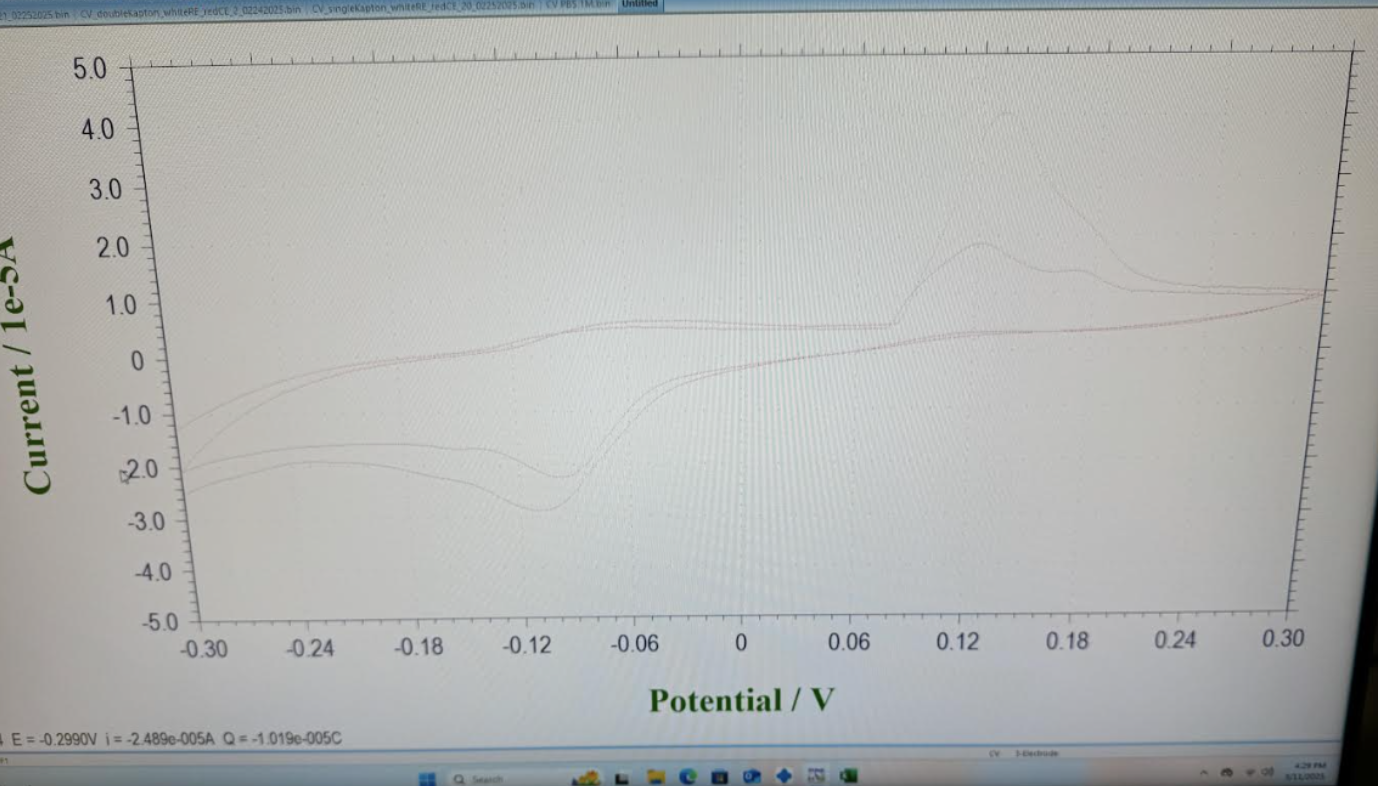
\includegraphics[width=0.45\linewidth]{fig9.png}
    \caption{Sensor 3 CV results}
    \label{fig}
\end{figure}

\smallskip

In the CV results for sensor 1, there are no distinguishable peaks, likely resulting from incomplete connections of one or a few of the electrodes. In the CV results for sensor 2, small peaks are visible, however there are two negative peaks, indicating there was some mixing of the silver ink. In the CV results for sensor 3, more distinct peaks can be seen, however two positive and negative peaks are present, again indicating reaction of the silver ink. 
\smallskip

\subsection{Microfluidics}
Three iterative designs of the microfluidic patch were tested using SimScale computational fluid dynamics (CFD) simulations. In the preliminary layout, the design included four inlets, a 15mm x 300µm x 300µm channel, and a 31mm x 5.6mm reservoir to house the sensor. Simulations indicated that old sweat would accumulate in the reservoir's corners. Additionally, sweat flow across the reservoir required approximately six minutes, making the design unsuitable for this project. The second design featured a modified 11mm x 6mm elliptical reservoir to accommodate the updated sensor layout, as well as a single inlet to prevent bubble formation. While sweat accumulation was prevented, flow time increased to nine minutes, and expanding the inlet size did not improve flow rate. The third design implemented the reservoir from design two, but reverted to the original four-inlet layout to speed up the flow rate. In this design, sweat did not accumulate and took roughly 2 minutes to cross the reservoir, suggesting that it may be suitable for our project.

\begin{figure}[hptb]
    \centering
    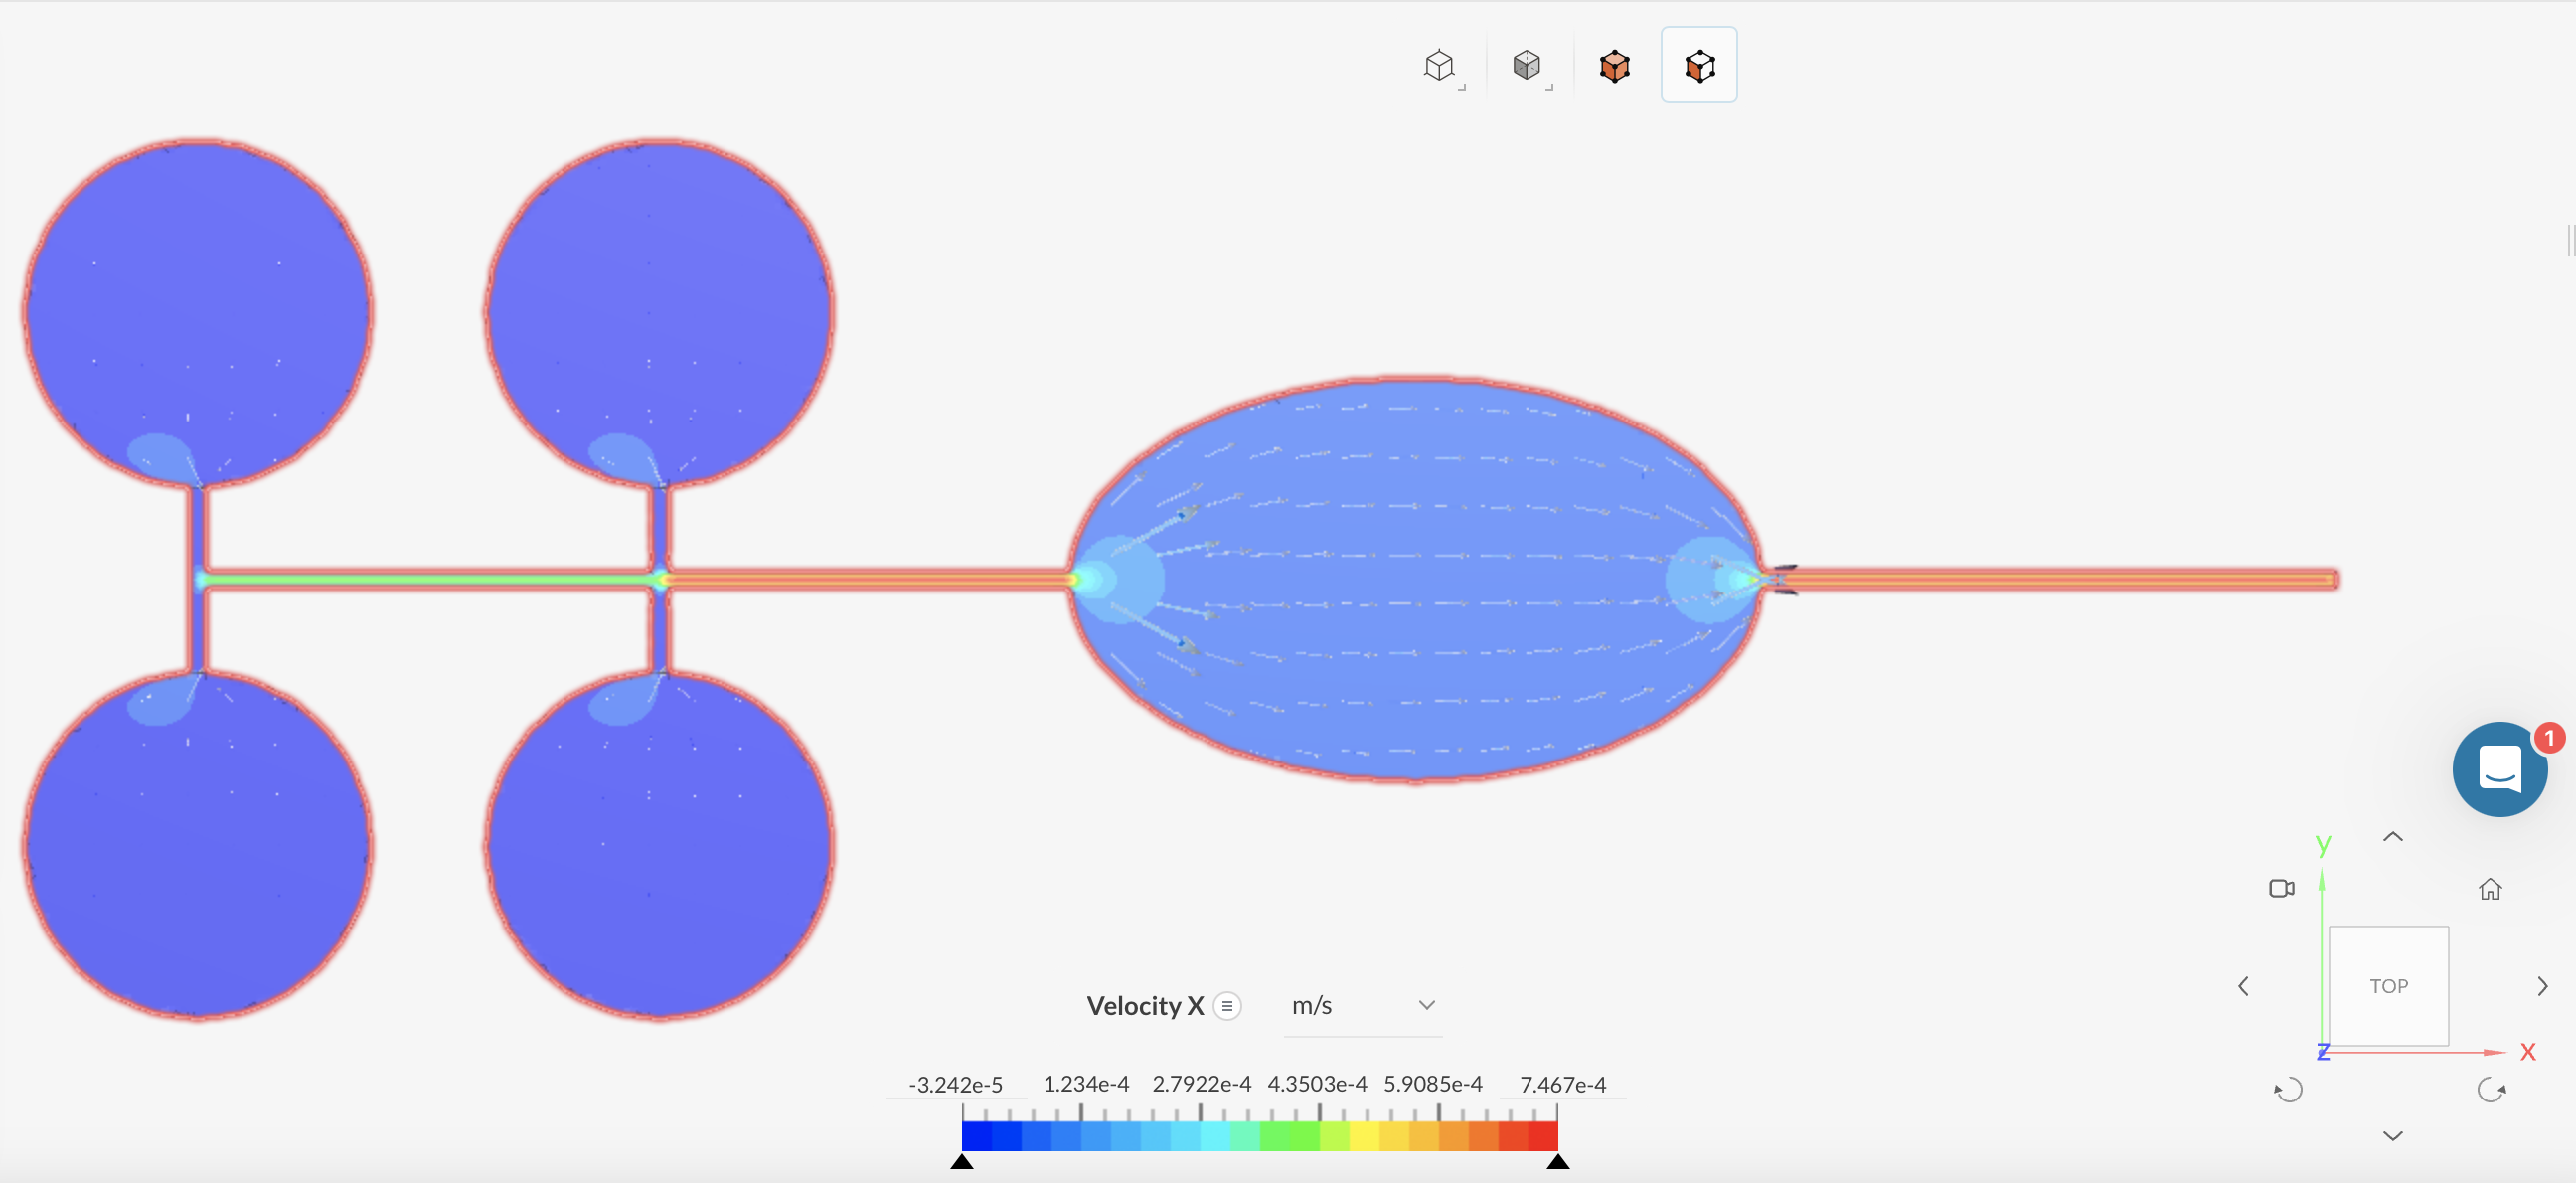
\includegraphics[width=0.45\linewidth]{fig10.png}
    \caption{Microfluidic Patch Design 3 Layout and CFD Simulation Results}
    \label{fig}
\end{figure}

The initial attempt to fabricate the microfluidic patch using PDMS was unsuccessful. Despite heating the molds for three hours at 70°C, the cured PDMS could not be extracted from the molds without breaking apart. 

\bigskip

\section{Discussion}
The prototype incorporates an 8-bit PWM signal, filtered by an RC network operating at approximately 31.4 kHz, producing an analog-like sweep with a potential window from –1V to 1V. ADC readings taken via a transimpedance amplifier circuit that converts the small currents generated at the counter electrode into measurable voltage levels. Overall, the prototype of a microcontroller-based potentiostat replicates the functions of a traditional, more expensive instrument and supports our low-cost design for continuous glucose or lactate monitoring. Also it provides a robust foundation for further integration onto a flexible PCB in continued development stages.

In the CV testing of the three sensors, it can be seen that there is contamination of the carbon signal with silver, shown by the two peaks instead of one in the graphs. Next steps to correct this is to apply the isolation solution more generously to all the silver parts of the sensor to ensure that there is no contamination. To further remove variables during CV testing, the working electrodes will be tested with control reference and counter electrodes. Once ideal CV graphs have been obtained, the working electrodes can then be modified with their respective enzymes and tested again. 

For the microfluidic patch, the team determined that an elliptical reservoir was crucial for avoiding sweat build up. It was also noted that using a 4-inlet layout was necessary to achieve the required speed across the reservoir. Additionally, the challenges faced when working with the molds and PDMS during fabrication suggest the need for an alternative method and materials. The team plans to use an LPKF laser to produce a more precise chip, as well as to modify the material used. Once fabricated, the patch will undergo testing with a syringe pump to verify the flow characteristics, and will then be integrated with the sensor for further testing.
\bigskip

\section{Acknowledgments} 

Thank you to Dr Moreto, Dr Sempionatto, Beatriz Mayol, and Julieta Nava Granados for their guidance and assistance during this project.

\bigskip

\section{References}
[1] Y. Yin, Z. Tan, W. Zhu, Z. Pu, H. Yu, R. Wang, and D. Li, "A wearable microfluidic system for efficient sweat collection and real-time detection," Talanta, vol. 274, p. 125967, 2024. [Online]. Available: https://doi.org/10.1016/j.talanta.2024.125967.



\end{document}
